\chapter{提案手法}
\label{cha:method}

本章では，本研究で提案する「髭密度を考慮した皮膚表面下散乱モデル」について詳述する。
本研究の目的は，人間の顔表面において局所的に分布する髭の影響を考慮し，
皮膚表面下散乱の見えをより現実的に再現することである。

本章では，まず本研究で扱う問題設定を整理し，
次にベースとなる皮膚表面下散乱モデルについて説明する。
その後，髭密度を導入した混合反射モデルと，
それを実現するための髭密度マップ生成手法を示す。
最後に，提案モデルをモンテカルロパストレーシングに統合する
レンダリングアルゴリズムについて説明する。

\subsection{問題設定}
本研究では，人間の顔表面における光輸送を対象とし，
特に髭が存在する領域において生じる表面下散乱の見えの変化に着目する。

従来の皮膚表面下散乱モデルでは，
皮膚を一様な多層媒質として近似する場合が多く，
局所的な構造物である髭の分布による影響は
明示的には考慮されてこなかった。
しかし実際の人間の顔では，
髭の密度は空間的に大きく変化しており，
これにより光の吸収量や散乱距離が領域ごとに異なる。
\begin{figure}[tb]
  \centering
  \subfloat[髭なし]{
    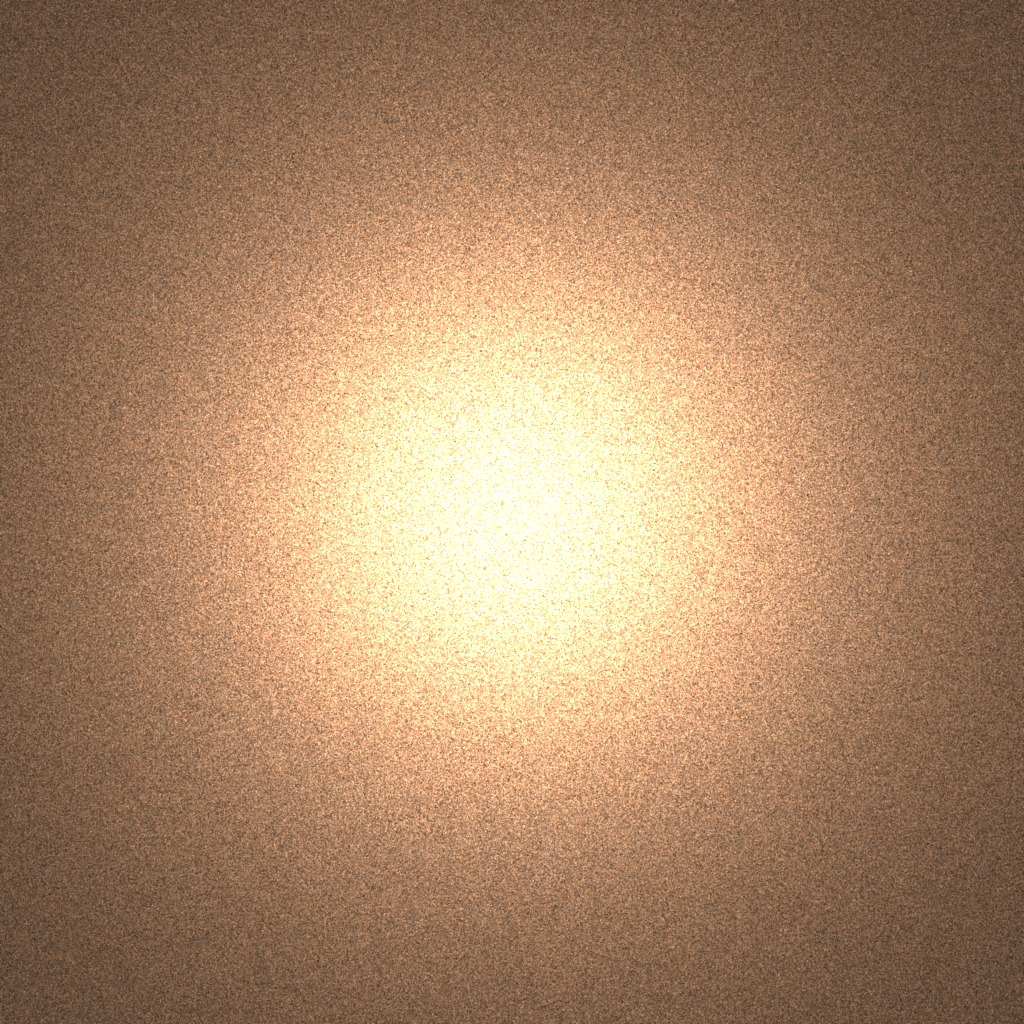
\includegraphics[width=0.46\linewidth]{figs/out_no_beard.png}
  }
  \hspace{0.04\linewidth}
  \subfloat[髭あり]{
    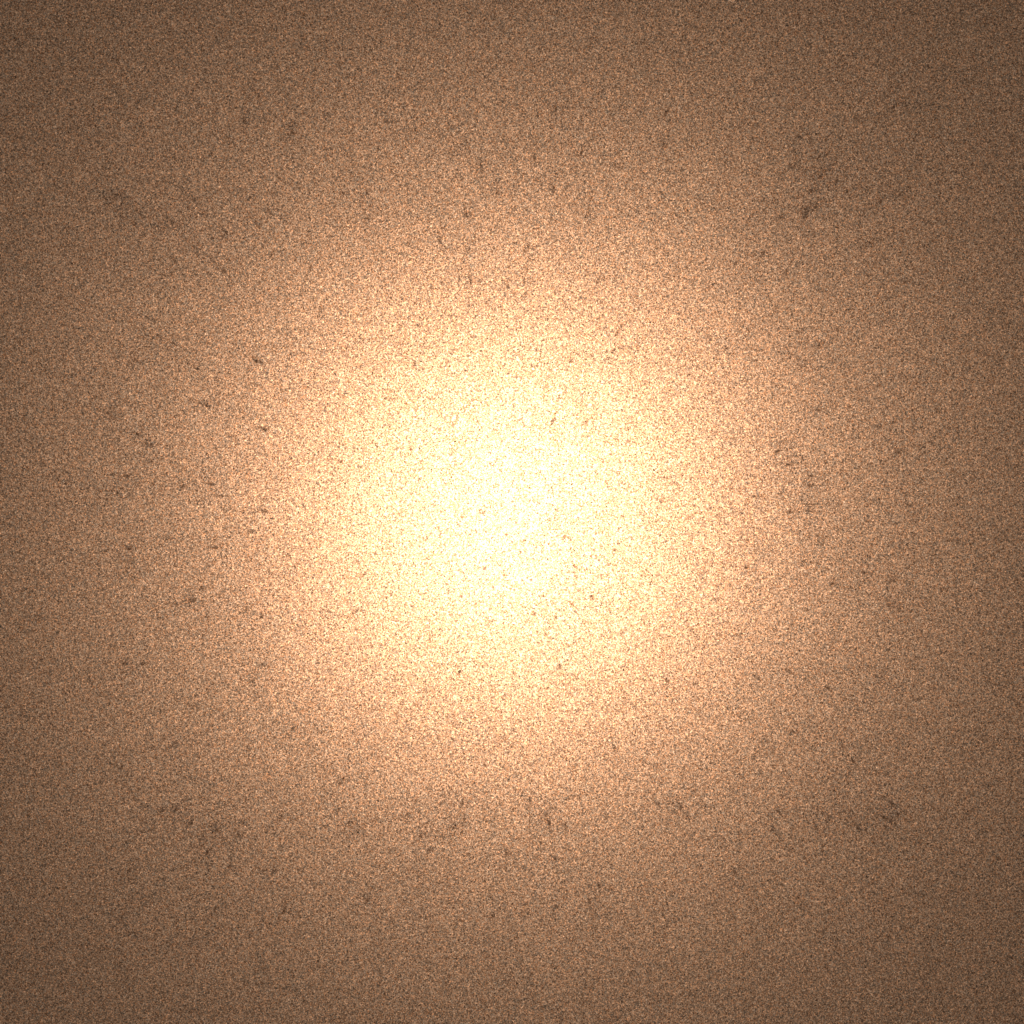
\includegraphics[width=0.46\linewidth]{figs/out_beard.png}
  }
  \caption{Mitsuba による髭なし／髭ありシーンのレンダリング結果。
髭が存在する領域では，皮膚のみの場合と比較して，
光のにじみや明度分布が変化する。}
  \label{fig:beard_effect}
\end{figure}

このような不均質性を無視したモデルでは，
髭の生えている領域において
光のにじみが過度に強く現れたり，
逆に暗部が不自然に減衰するなどの問題が生じる。
そこで本研究では，
皮膚表面下散乱モデルに髭密度という空間的に変化するパラメータを導入し，
髭の存在による影響を連続的に表現することを目的とする。

\subsection{皮膚表面下散乱モデル}
皮膚内部における光の散乱は，
光が表面から入射し，内部で複数回散乱した後，
異なる位置から出射する現象として観測される。
このような光輸送を記述するため，
本研究では双方向表面下散乱反射率分布関数
(Bidirectional Surface Scattering Reflectance Distribution Function: BSSRDF)
を用いる。

BSSRDF は，入射位置 $\mathbf{x}_i$，
入射方向 $\omega_i$，
出射位置 $\mathbf{x}_o$，
出射方向 $\omega_o$ に依存する関数として定義され，
次式で表される。

\begin{equation}
S(\mathbf{x}_i, \omega_i, \mathbf{x}_o, \omega_o)
=
\frac{dL_o(\mathbf{x}_o, \omega_o)}
     {d\Phi_i(\mathbf{x}_i, \omega_i)}
\end{equation}


本研究では，
既存研究において広く利用されている
拡散近似に基づく皮膚BSSRDFモデルをベースモデルとして採用する。
拡散近似は，
散乱回数が十分に多い場合に成立する近似であり，
人間の皮膚のような強散乱媒質に対して
計算効率と再現性の両立が可能である。


\subsection{髭密度を考慮した混合モデル}
髭が存在する皮膚表面では，
皮膚のみの場合と比較して，
光の吸収および散乱特性が変化する。
髭は主にメラニンを多く含む毛髪繊維で構成されており，
皮膚表面付近において光を吸収・遮蔽する役割を果たす。

本研究では，
この影響を明示的にモデル化するため，
皮膚モデルと髭モデルを
髭密度に基づいて混合する手法を提案する。
各表面点において髭密度を
$d \in [0,1]$ と定義し，
$d=0$ は髭の存在しない皮膚，
$d=1$ は髭の影響が最大である状態を表す。

出射点における表面下散乱特性は，
次式に示すように，
皮膚モデルと髭モデルの線形結合として表現される。

\begin{equation}
S_{\mathrm{mix}}
=
(1 - d)\, S_{\mathrm{skin}} + d\, S_{\mathrm{beard}}
\end{equation}

線形混合を採用した理由は，
髭密度が連続的に変化する領域において，
反射特性が不連続に変化することを防ぎ，
安定したレンダリング結果を得るためである。
また，本手法は既存のBSSRDFモデルを拡張する形で実装可能であり，
計算コストの増加を最小限に抑えられるという利点を持つ。
\subsubsection{髭密度を出射点で評価する理由}
本研究では，髭密度 $d$ を入射点ではなく，
表面下散乱後の出射点において評価する。
これは，本研究で用いるBSSRDFが，
光の入射位置と出射位置が異なる現象を記述するモデルであり，
最終的な見えに直接影響を与えるのが出射点であるためである。

皮膚表面下散乱では，
光は皮膚内部を伝播した後，
周囲の別の位置から出射する。
そのため，入射点近傍における髭の有無よりも，
実際に光が出射する位置周辺の構造が，
最終的な放射輝度に強く影響する。

仮に入射点の髭密度のみを用いた場合，
皮膚内部で大きく移動した光に対しても，
入射点の情報が適用されることになり，
髭分布と見えの対応関係が不自然になる可能性がある。
特に，髭の境界付近では，
入射点と出射点で密度が大きく異なる場合があり，
これがアーティファクトの原因となる。

以上の理由から，本研究では，
表面下散乱サンプリングによって決定された出射点において
髭密度を参照し，
混合反射モデルを適用する設計とした。
\subsubsection{髭モデルの反射特性}
本研究における髭モデル $S_{\mathrm{beard}}$ は，
髭一本一本の幾何構造を直接表現するものではなく，
髭の存在によって生じる
皮膚表面下散乱特性の変化を近似的に表現するモデルである。

髭は皮膚表面付近に分布する毛髪繊維であり，
光に対して主に吸収および遮蔽の役割を果たす。
その結果，髭が存在する領域では，
皮膚内部を長距離伝播する光の寄与が減少し，
有効的な散乱距離が短くなる傾向がある。

本研究では，
この効果を簡潔に表現するため，
髭モデルを
皮膚モデルと比較して
吸収の強い，
かつ拡散半径の小さい反射モデルとして定義する。
これにより，
髭密度が高い領域では，
表面下散乱による光のにじみが抑制され，
より引き締まった見えが得られる。

このように，
$S_{\mathrm{beard}}$ は
毛髪一本単位の物理モデルではなく，
皮膚表面下散乱に対する
髭の影響を集約的に表現する
有効モデルとして位置づけられる。

\subsubsection{線形混合モデルにおける近似と限界}
本研究で採用した混合モデルは，
髭密度 $d$ に基づいて皮膚モデルと髭モデルを線形に補間するものである。
この定式化は実装が容易であり，
既存の表面下散乱モデルとの親和性が高い一方で，
いくつかの近似を含んでいる。

まず，本研究では，
髭一本一本の物理的形状，
すなわち太さ，長さ，曲率，および生え方の方向分布といった
高次の幾何学的要因を明示的には考慮していない。
実際の髭は円柱状の繊維構造を持ち，
その太さや長さは光の遮蔽率や散乱特性に影響を与える。
しかし，これらの要因を直接モデル化するためには，
毛髪一本単位でのジオメトリ表現や，
異方的な散乱モデルを導入する必要があり，
計算コストが著しく増大する。

また，髭同士の重なりによる自己遮蔽や，
毛髪間で生じる多重散乱効果も本研究では考慮していない。
これらの効果は，
高密度な髭領域において特に重要となるが，
正確に扱うためには，
毛髪集合体を体積媒質として扱うような
高度なモデルが必要となる。

本研究では，
これらの高次効果をすべて
髭密度という単一のスカラー量に集約することで，
皮膚表面下散乱に対する髭の影響を
低次元かつ連続的に表現することを選択した。
この近似により，
レンダリングの安定性を保ちつつ，
髭分布に応じた見えの変化を
実用的な計算時間で再現することが可能となる。

以上より，本研究の線形混合モデルは，
物理的に厳密な毛髪モデルではなく，
皮膚表面下散乱への影響を簡潔に取り込むための
近似モデルとして位置づけられる。
\subsubsection{他の混合モデルとの比較}
髭密度に基づく反射モデルの構築にあたり，
線形混合以外の手法についても検討を行った。
例えば，
非線形関数による補間や，
指数関数を用いた減衰モデル，
あるいは有効散乱係数を
髭密度に応じて直接変化させる手法が考えられる。

しかし，非線形混合モデルでは，
髭密度のわずかな変化に対して
反射特性が急激に変化する場合があり，
密度分布が滑らかな領域においても
不安定なレンダリング結果を生じることが確認された。
また，有効散乱係数を直接操作する手法では，
物理パラメータの解釈が困難となり，
既存の皮膚表面下散乱モデルとの比較が難しくなる。

これに対して，
線形混合モデルは，
髭密度と反射特性の関係が直感的であり，
密度が連続的に変化する場合でも
安定した結果を得ることができる。
以上の理由から，
本研究では線形混合モデルを採用した。


\subsection{髭密度マップの生成}
髭密度は，
顔表面上の各位置に対して定義されるスカラー量であり，
テクスチャマップとして表現される。
本研究では，
髭ジオメトリの分布情報から
密度マップを自動生成する。

\begin{figure}[tb]
  \centering
  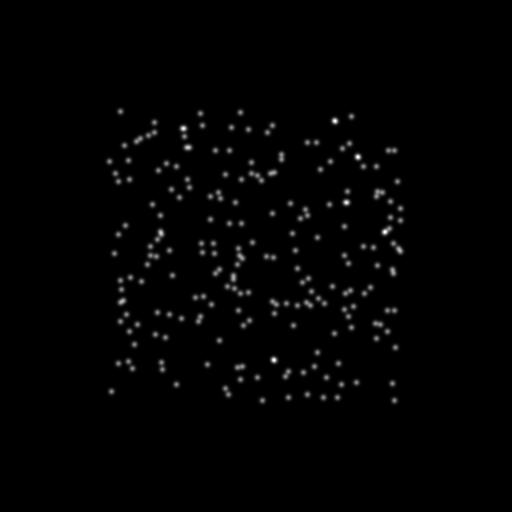
\includegraphics[width=0.8\linewidth]{figs/beard_density_xz.jpg}
\caption{髭ジオメトリから生成された髭密度マップの例。
密度マップはUV空間上に定義され，
レンダリング時に各表面位置の密度値を取得するために用いられる。}



  \label{fig:beard_density_map}
\end{figure}
まず，髭ジオメトリを入力として，
各皮膚表面点に対する近傍領域を定義する。
次に，その領域内に含まれる髭の本数や占有率を評価し，
正規化された密度値として $d$ を算出する。
生成された密度値はUV空間に投影され，
テクスチャマップとして保存される。

この密度マップは，
レンダリング時において
表面位置に対応する密度値を高速に取得するために用いられる。
\subsubsection{密度マップの解像度と平滑化処理}
髭密度マップの解像度は，
見えの再現性と計算効率の両立において
重要な要素である。
解像度が低すぎる場合，
髭分布の境界が粗くなり，
表面下散乱結果に
ブロック状のアーティファクトが生じる。
一方で，過度に高解像度な密度マップは，
メモリ使用量の増加や
キャッシュ効率の低下を招く。

本研究では，
これらのトレードオフを考慮し，
実験的に十分な精度が得られる解像度を採用した。
また，密度マップ生成時には，
局所的なばらつきを抑制するため，
平滑化処理を施している。
この処理により，
髭の疎密が連続的に変化する領域においても，
自然な見えを維持することが可能となる。

なお，密度マップは
髭ジオメトリに基づく近似であるため，
完全に正確な物理量ではない。
しかし，本研究では，
この近似が視覚的な品質に与える影響は限定的であり，
提案手法の有効性を評価する上で
十分であると判断した。

\subsection{レンダリングアルゴリズム}
提案手法を用いたレンダリングは，
モンテカルロ法に基づくパストレーシングによって行う。
出射放射輝度は次式により数値的に推定される。

\begin{equation}
L_o(\mathbf{x}_o, \omega_o)
\approx
\frac{1}{N}
\sum_{k=1}^{N}
\frac{f_k\, L_i(\omega_k)\, \cos\theta_k}
     {p(\omega_k)}
\end{equation}

本研究では，
この推定を表面下散乱サンプリングに組み込み，
サンプリングされた出射点において
髭密度を参照することで，
混合BSSRDFを適用する。

提案手法を用いたレンダリングの処理手順を以下に示す。

\begin{enumerate}
  \item レイと皮膚表面との交差判定
  \item 交差点における髭密度の取得
  \item 髭密度に基づく混合反射モデルの決定
  \item 表面下散乱に基づく出射点サンプリング
  \item 放射輝度の計算
\end{enumerate}

以上の処理を
モンテカルロパストレーシングに統合することで，
髭密度に応じた表面下散乱表現を実現する。
\subsection{計算コストと実装上の考察}
提案手法では，
髭密度マップの参照と
混合反射モデルの計算が追加されるが，
これらはいずれも定数時間で実行可能である。
そのため，
レンダリング全体の計算量は，
従来のBSSRDFを用いたパストレーシングと
同程度に保たれる。

特に，
髭をジオメトリとして直接扱わず，
密度マップとして集約した点は，
計算量削減の観点から重要である。
毛髪一本単位の交差判定や散乱計算を行う場合と比較して，
提案手法は
実用的な計算時間でのレンダリングを可能にする。
